\documentclass[]{report} 
\usepackage{wrapfig}
\usepackage{float}

% Graphics pacakges
\ifx\pdfoutput\undefined
  % we are running LaTeX, not pdflatex
  \usepackage{graphicx}
\else
  % we are running pdflatex, so convert .eps files to .pdf
  \usepackage[pdftex]{graphicx}
  \usepackage{epstopdf}
\fi

\begin{document}

\title{Amazon Review Sentiment Analysis} 
\author{Alan J. Perez-Rathke \and Gary I. Turovsky}
\date{April 28, 2011}   
\maketitle


\section{Introduction} 
There are quite a few unsolved problems in the field of data mining.  But sentiment analysis presents us with a special challenge.  Sentiments are subtle and context-dependent.  They demand a depth of understanding of the underlying meaning that even the state-of-the-art can't provide.

But, of course, such information has value. For example,it would be handy for a product manufacturer to automatically collect sentiment data about its product.  This can help improve the product and direct advertising efforts.

Amazon is a large online retailer which naturally has such product sentiment data.  For some of the more popular products they carry, people post reviews - and often people reply to such reviews with comments.  We were given the specific problem of classifying these comments into two classes.  One class was to contain the comments which expressed some opinion about the product review.  And the other class contained those comments which did not.  See the accompanying figure for an example from each class.


\begin{figure}[h]
	\begin{center}
		\begin{tabular}{ p{5 cm}  p{5 cm} }
			\begin{center}Sentimental Review\end{center} & 
			\begin{center}Non-sentimental Review\end{center}\\
			Great review, all of the information is really helpful and I think you and your wife helped me in making my decision! I am ordering my Kindle 3 very soon, thanks!
			& 
			Question - I saw on your cover review that you got both the grey and the white versions. Which one do you prefer and how much difference is there between the two?  \\
		\end{tabular}
	\end{center}
	\caption{Examples from the two classes of reviews}
	\label{figExampleReviews}
\end{figure}

We believed that the simplest approach would be the best approach here.  At least at first, we did not want to create a new type of classifier.  We wanted to use known classifiers to create a baseline from which to improve our results. 

\section{Techniques Used}

During our initial brainstorms about this problem we decided to focus on writing our program to construct a generic feature vector which we would run through several classifiers.  We discussed using naive bayes, SVM, and decision trees.  As it turned out, naive bayes gave us the best and most consistent results.  Initial implementations that used the decision tree were discouraging and we stopped experimenting with it early on.  Only SVM and naive bayes were consistently experimented with.  Though, almost every time naive bayes performed best for us.  So, all results we will discuss were achieved by using a naive bayes classifier.

The first and most obvious thing to try was to work out which single words in the comments signalled some opinion about the review.  We collected all the single words from each review and this turned out to be a set that numbered in the thousands.  This was far too large to be our features so we decided to arbitrarily grab the first few hundred.  

There were a few words with the same root among the features, so we started to stem the words before adding them to the feature vector.  In addition, we removed all punctuation.  This gave us a surprisingly high baseline of approximately 70\%.

It seemed that we should care more about comments which had phrases like "great review" in the text.  This gave us the idea of paying attention to nouns and adjectives only.  We filtered our feature vector to include only the single words which were nouns and adjectives.  Now "great" and "review" (along with words like "thanks" and "informative") came up near the top of the most helpful features for classification.  We wanted to make sure to capture any occurence of the two words together now so we started merging the most common single words into phrases whenever they occured next to each other.  That is, if the adjectvie "great" occured in a sentence and then the next noun word in the sentence was "review", we counted that as the feature "great review".  This allowed us to also count the sentences "great review" and "review was great" as the same (as word order didn't matter in our analysis either).  We also made the fact that a review started with a word to be a feature in itself.

\begin{figure}
	\begin{center}
	\begin{tabular}{ p{7 cm} | p{3 cm} }
			Feature& 
			Class     \\
			\hline
			\hline
			Phrase: "great review" & Sentimental  \\
			\hline
			Phrase: "thank time" & Sentimental  \\
			\hline
			Number of comments by user: 1, Words: "thanks" and "review", Starts with: "thank" & Sentimental \\
			\hline
			Number of comments by user: 1, Words: "review", Starts with: "thank" & Sentimental \\
			\hline
			Phrase: "help review" & Sentimental  \\
			\hline
			Phrase: "review thank" & Sentimental  \\
			\hline
			Comment author is review author & Non-sentimental  \\
			\hline
			Word: "delet" & Non-Sentimental  \\
			\hline
			Starts with: "excel" & Sentimental  \\
			\hline
		\end{tabular}
	\end{center}
	\caption{Ten of the typically most useful features in our feature set}
	\label{figBestFeatures}
\end{figure}


This improved our accuracy but we were still getting garbage phrases in our feature vector, such as "ipod nano", which clearly would only help discriminate for particular reviews.  We needed to focus on the most important phrases and words.  For this, we decided to use a tf-idf score for each word and phrase.  Strangely, this introduced a lot of garbage words and phrases into our feature vector and eliminated others that we thought would be good discriminators.  We decided to compare this to a straight threshhold.  That is, we would only consider words and phrases that occured in response to several different reviews.  Experimentally, we settled on a threshhold of about 30\% of the reviews.  This worked a lot better to eliminate extraneous features than the tf-idf score.

At this point, incorporating the hepfulness of a review, the length of a review, and the frequency of a commenter in a comment thread were added to the feature vector but had very little effect on the accuracy.  We also tried to see whether a review's star rating for a product was different from that product's average star rating.  Perhaps the comments in such a review are more likely to feel one way or another about the review, but it had little effect on the accuracy. One feature which worked was whether the author of a comment was the author of the review (since authors will rarely express any feeling about how good or bad their review was).

Here we ran into the dilemma of where to go next.  In our testing, we were hovering around 75\% accuracy on average.  To do any better, it would seem we would need a new approach.  But switching to another technique seemed risky.  Was there some other way of improving the naive bayes classifier?

Since there is an intrinsic assumption of conditional independence in the naive bayes approach, we knew we were missing some features which, together, could be important.  In order to find these, we decided to use the CAR algorithm.  For each class, we extracted the features that co-occured together and used the fact that these co-occur as a feature in itself to add to the feature vector.  For example, it turned out to be informative when there was only a single comment from a certain user and they started this comment with the word "great".  This was far more significant than the two features separately.

We made one more attempt to improve the feature vector.  We attempted to create two clusters out of the feature vectors.  Once we found the mean of both clusters, we added a feature to each feature vector with the standard deviation from the mean.  This, unfortunately, did not help our accuracy, so we removed these features from our feature vector when doing the final classification.

One final note here about using an SVM for classification.  We used the libsvm package which comes with a handy little python script which makes the classification process "fool-proof".  This script first estimates parameters for an rbf kernel before doing the actual classification.  Each such run took a much longer time than the naive bayes classifier (which made working on improving this classifier quite a bit more difficult) and it also never outperformed the naive bayes classifier, besides being inconsistent to boot.  We saw accuracies of anywhere between 60\% and 80\%, which we thought would not be acceptable if we were to be competitive with the other teams.  We really wanted the SVM to work, but it would always disappoint.

\section{Experiments}

In the interest of determining which features were most valuable, we ran several experiments to see how each contributed to the final accuracy of the classifier.  First, we ran the classifier using only a base feature set: whether or not a word exists within a comment.  We then ran the classifier using the base feature set combined with only a single other set.  The results of these experiments are shown in Figure \ref{fig:MinimalFeatureSets}.  From this, we can see that many of the additional features, such as helpfulness ratio, appear to actually be detrimental to the final accuracy.  Furthermore, we can immediately see that 2-word phrases (also referred to as 2-gram phrases) and CAR mining significantly increase accuracy.
\begin{figure}[H]
\centering
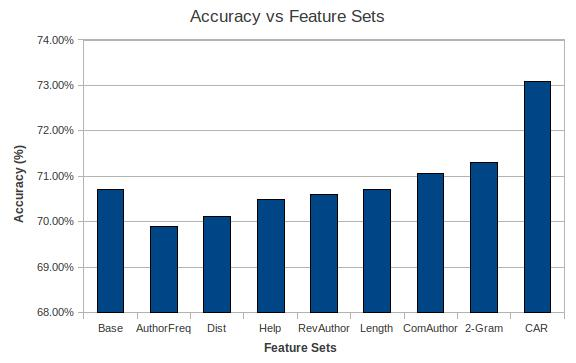
\includegraphics[width=3.77in]{AccuracyVsFeatureSets.jpg}
\caption{The resulting accuracies when only a single feature set is combined with the base feature set.  The base feature set consists only of whether or not a word exists in a comment.}
\label{fig:MinimalFeatureSets}
\end{figure}

Next, we ran a series of experiments that combined multiple feature sets.  The results can be seen in Figure \ref{fig:MultiFeatureSets}.  From this, we can see that, without using CAR mining, the maximum  accuracy remains at just over 71\%.  However, with the addition of CAR features, the accuracy jumps to just over 76.5\%.  Furthermore, the boost from CAR mining is dependent on the existence of the "2-gram phrases" and ''Author frequency in review" feature sets (which contain whether or not the commentor has posted before and if the author of a review is commenting).  From this, we can see that our highest quality is achieved by solely using these feature sets - inclusion of additional feature sets only reduces quality.

\begin{figure}[H]
\centering
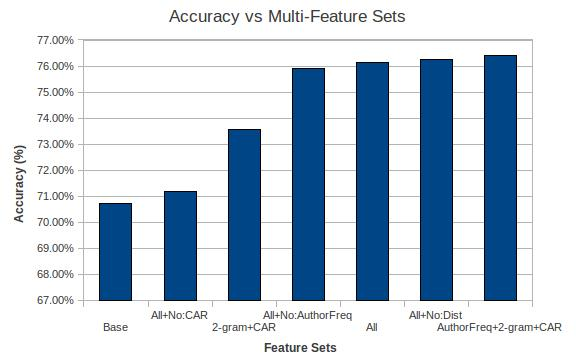
\includegraphics[width=3.77in]{AccuracyVsMultiFeatureSets.jpg}
\caption{The resulting accuracies when only multiple feature sets are combined with the base feature set.}
\label{fig:MultiFeatureSets}
\end{figure}

The ''2-gram phrases" features set, which consists of adjective and noun pairs that appear consecutively within a comment, has proven to be one of the most valuable sets in terms of accuracy.  From Figure \ref{fig:WordCountSupport}, we can see how accuracy is influenced by the minimum support (i.e. how often a word appears in different reviews) for words allowed in the pairings.  When the minimum support is below 30\%, too many misleading phrases are generated and the accuracy suffers.  In contrast, when the minimum support is above 30\%, too few phrases are generated and again the accuracy pays a penalty.  From this data, we can conclude that 30\% is a near optimal setting for support threshhold. 

\begin{figure}[H]
\centering
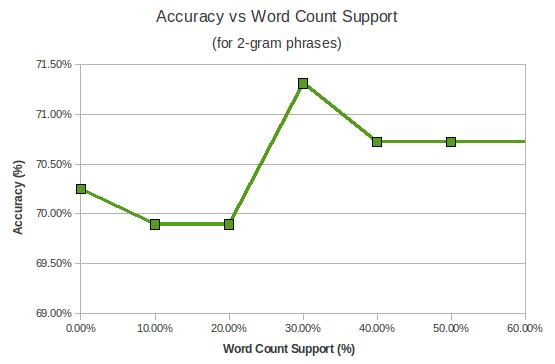
\includegraphics[width=3.77in]{AccuracyVsWordCountSupport.jpg}
\caption{The resulting accuracies when word count support is varied.  Accuracies are the result of the base feature set combined with 2-gram phrases.}
\label{fig:WordCountSupport}
\end{figure}


Other parameters of interest include CAR minimum support and minimum confidence threshholds.  From Figure \ref{fig:CARMinSup}, we can see that accuracy peaks when the minimum support threshhold is at 10\%.  We can surmise that lower values generate too many CAR associations and high values generate too few associations; therefore, both of these cases result in a decline in accuracy.  A similar analysis can be done for CAR minimum confidence as shown in Figure \ref{fig:CARMinConf}.  We can see that when minimum confidence is below 58\% or above 61\%, accuracy declines from either too many or too few associations respectively. 


\begin{figure}[h]
\centering
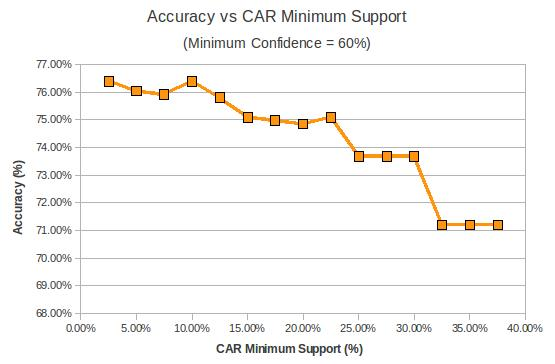
\includegraphics[width=3.77in]{AccuracyVsCARMinimumSupport.jpg}
\caption{The resulting accuracies when the minimum support for CAR mining is varied.  Accuracies are the result of the base feature set combined with 2-gram phrases and author frequencies.}
\label{fig:CARMinSup}
\end{figure}

\begin{figure}[H]
\centering
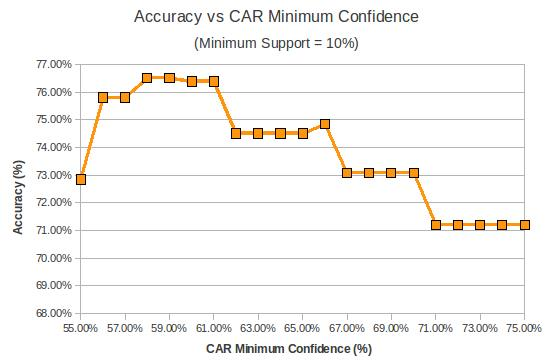
\includegraphics[width=3.77in]{AccuracyVsCARMinimumConfidence.jpg}
\caption{The resulting accuracies when the minimum confidence for CAR mining is varied.  Accuracies are the result of the base feature set combined with 2-gram phrases and author frequencies.}
\label{fig:CARMinConf}
\end{figure}

\section{Conclusion and Further Work}
Our work on this project has mainly revolved around creating the optimum feature vector such that a naive bayes classifier would be able to better discriminate between the two classes.  In a way this is a bit of a boring approach and it would have felt a lot better to find something more interesting and innovative that did far better.  Without having a good way to understand language, this seemed like a daunting task.  In order to really understand sentiment, we have to be able to extract meaning from a text.  One could even venture to say that in a lot of ways, knowing the feeling in a sentence is a huge step towards understanding its meaning.

In the course of working on this project, it is unfortunate that we could never be consistently accurate with an SVM.  It seemed, by all accounts we were aware, that an SVM would be perfect for dealing with text data.  Perhaps further tweaking or using a different kernel could have yielded better results.  Maybe a simpler kernel could have also reduced the training time.

It also seems that we could have taken more risks.  Something interesting to try would be a sort of Hidden Markov Model approach.  Let's say that, in our HMM, each word is a state.  It has a transition probability between it and another state that depends on how often these words co-occur in a sentence.  The observation for each state would be the word for each state.

Two HMMs could be trained.  One for comments with sentiments about the review and one for comments without sentiments about the review.  When doing the testing, the classifier would calculate which HMM the word sequence was most likely to come from.  Such a set of models might also be interesting since we could use them to generate examples of comments from either class.

We certainly feel we could have done a lot better if we had gone into it knowing what we know now about the problem.  Our ultimate goal was to get into the 80\% range, but we never managed to do it.  That would have given us greater confidence about our approach and made winning the class contest a bit sweeter.  Despite this, it is our opinion that we managed to squeeze out an impressive amount of accuracy from a naive bayes classifier, and this has some merit.



\end{document}
